\apendice{Documentación de usuario}

\section{Introducción}

En este Apéndice se resumirá como interaccionar con la interfaz web que da acceso al conjunto de datos curado.

\section{Requisitos e Instalación}

Al tratarse de una aplicación web al uso, el usuario simplemente debe acceder con cualquier navegador con JavaScript activo (Chrome, Firefox, Edge...) al dominio \href{https://www.buscahogar.es}{buscahogar.es}.

\clearpage
\section{Manual del usuario}

En esta sección se detallará como interactuar con las distintas vistas del sitio web: \texttt{INICIO}, \texttt{EXPLORA}, \texttt{VISUALIZA} e \texttt{INFO}. Tras acceder a la página, lo que vemos se observa en la Figura \ref{fig:inicio_0}



Se puede acceder a las distintas vistas del sitio web a través de la barra de navegación, mostrada en la parte superior derecha de la Figura~\ref{fig:inicio_0}. En dicha barra de navegación, la vista seleccionada se remarca en color azul.

\begin{figure}[ht]
    \centering
	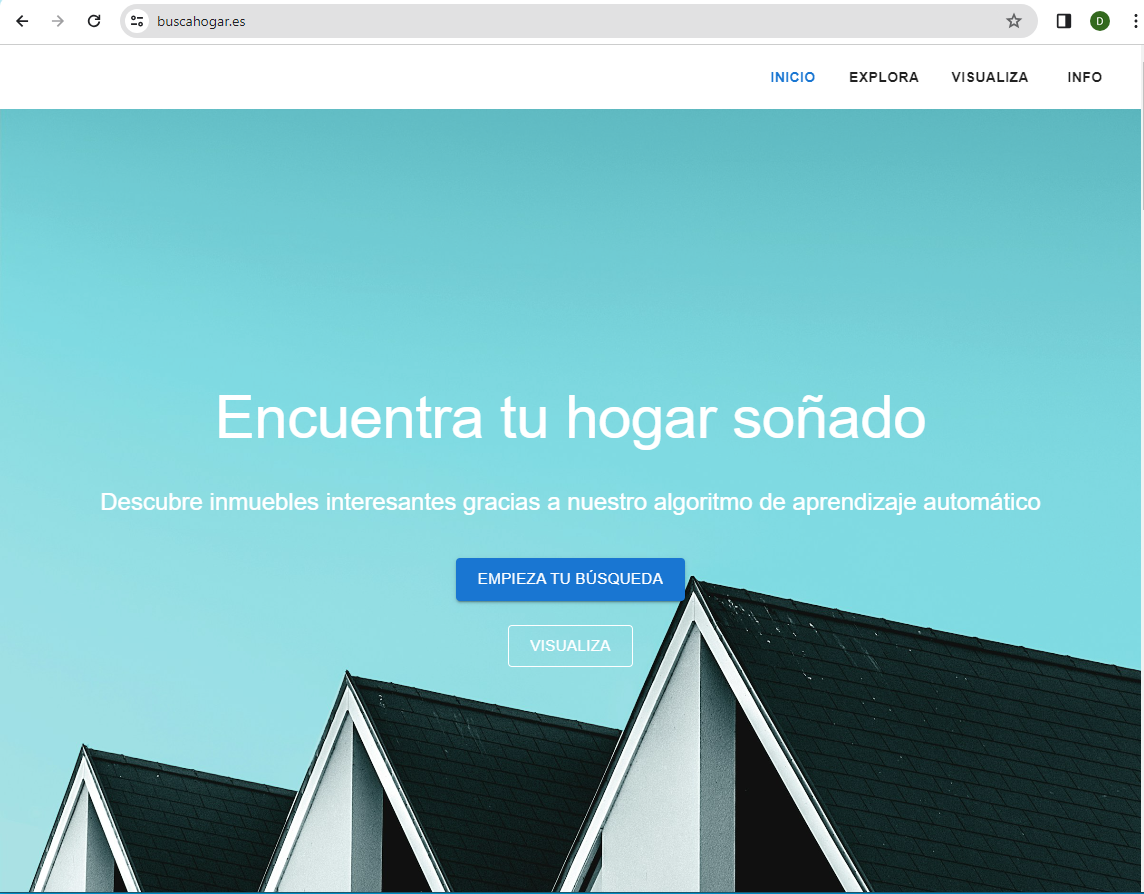
\includegraphics[width=1\textwidth]{img/inicio_0.PNG}
	\caption[Página de inicio \url{www.buscahogar.es}]{Página de inicio \url{www.buscahogar.es}, en la parte superior derecha vemos la barra de navegación}
	\label{fig:inicio_0}
\end{figure}

\begin{figure}[ht]
    \centering
	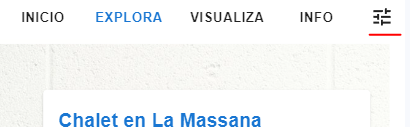
\includegraphics[width=1\textwidth]{img/filtro_replegado_1.PNG}
	\caption[Barra de navegación de \url{www.buscahogar.es} en pantallas móviles]{Barra de navegación de \url{www.buscahogar.es} en pantallas móviles. Al pulsar el botón marcado en rojo se despliegan los filtros de las pestañas \texttt{INICIO}, \texttt{EXPLORA} y \texttt{VISUALIZA}.}
	\label{fig:filtro_moviles}
\end{figure}

\clearpage
\subsection{INICIO}{\label{sec:web_inicio}}

En esta vista se muestra la página de inicio, que hace la función de ventana de \textit{marketing} para el resto del portal. Tras unos breves textos de ``llamada a la acción'', encontramos una sección con funcionalidad que merece la pena explicar (Ver Figura \ref{fig:inicio_1}): 

En esta sección se muestran los inmuebles con mayor puntuación asignada por los modelos para las provincias seleccionadas (Ver calculo en Sección \ref{sec:ml_section}). Por defecto, aparecen los cinco inmuebles de mayor puntuación para todas las provincias y además, el modo inteligente (\textit{Smart Mode}) se encuentra  activado. Este modo limita la puntuación máxima a 0.4 (Lo que significa que los modelos le asignan un 40\% más de precio que el de venta), ya que se ha observado que inmuebles con más de esa puntuación suelen ser falsos positivos.

Por lo tanto, encontramos tres selectores: (1) Provincia, (2) Si queremos inmuebles solo en capital de provincia, (3) Modo Inteligente (limitación a 0.4 de puntuación máxima). Además, encontramos botón de interrogación que explica en qué consiste el modo inteligente. Estos selectores se repliegan en pantallas móviles, para desplegarlos hay que pulsar el icono de filtro en la parte superior derecha (ver Figura \ref{fig:filtro_moviles}).


\begin{figure}[ht]
    \centering
	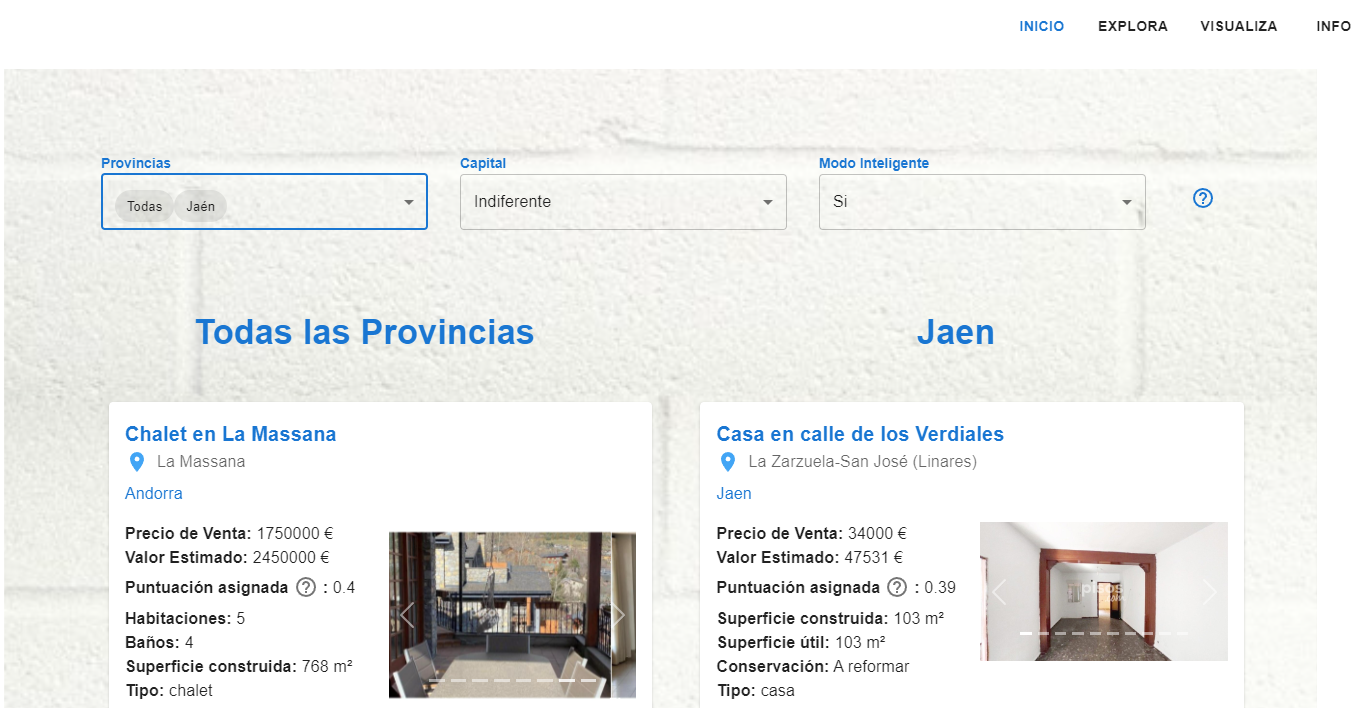
\includegraphics[width=1\textwidth]{img/inicio_1.PNG}
	\caption[Parte inferior de la página de INICIO en \url{www.buscahogar.es}]{Parte inferior de la página de INICIO en \url{www.buscahogar.es} con provincia ``Todas'' y ``Jaen'' seleccionadas}
	\label{fig:inicio_1}
\end{figure}

\clearpage
\subsection{EXPLORA}{\label{sec:web_explora}}

En esta sección, que representa el núcleo de la web, encontramos el acceso al listado de todos los inmuebles en la base de datos. En la parte izquierda encontramos los filtros y en la derecha el listado de inmuebles (Ver Figura \ref{fig:explora_1}. En pantallas móviles o de pequeño tamaño, los filtros de la parte izquierda se repliegan, para desplegarlos hay que pulsar el icono de filtro en la parte superior derecha (Ver Figura \ref{fig:filtro_moviles}).

Por defecto, los inmuebles están organizados en orden de puntuación descendente, con un máximo de 0.4 (equivalente al modo Inteligente, explicado en Sección \ref{sec:web_inicio}. Todos los inmuebles listados incluyen los datos originales listados en \url{www.pisos.com}, y además el valor estimado por los modelos de Aprendizaje Automático, junto con la puntuación (Para ver como se calcula ver \ref{sec:ml_section}), además de un botón con forma de interrogación que explica la puntuación asignada.

Los filtros, desde la parte superior a la inferior, son los siguientes:

\begin{itemize}
    \item Provincia: La Provincia de la que quieres ver inmuebles
    \item Capital: Si quieres ver inmuebles solo en la capital de Provincia, fuera de la capital o indiferente.
    \item Tipo: El tipo de inmueble, puede ser indiferente. Piso, casa, apartamento...
    \item Precio (\textit{Slider}): El rango de precios (en €) que queremos ver. Se trata del precio de venta real del inmueble.
    \item Habitaciones (\textit{Slider}): Los inmuebles que se mostrarán estarán en ese rango de número de habitaciones que queremos ver.
    \item M2 Útiles (\textit{Slider}):  Los inmuebles que se mostrarán estarán en ese rango de metros cuadrados útiles que queremos ver.
    \item Puntuación (\textit{Slider}): Los inmuebles que se mostrarán estarán en ese rango de puntuaciones (asignadas por Aprendizaje Automático)
    \item Ordenar por: La forma en la que quieres ordenar el listado, por defecto en puntuación descendente. 
\end{itemize}

De forma interesante, la pestaña explora no incorpora paginación como suele ocurrir en los portales inmobiliarios comunes, se ha implementado un mecanismo de \textit{scroll} infinito similar al de la mayoría de redes sociales, en el que se van cargando inmuebles que cumplen las especificaciones del filtro a medida que el usuario alcanza el límite inferior de la página.

\begin{figure}[ht]
    \centering
	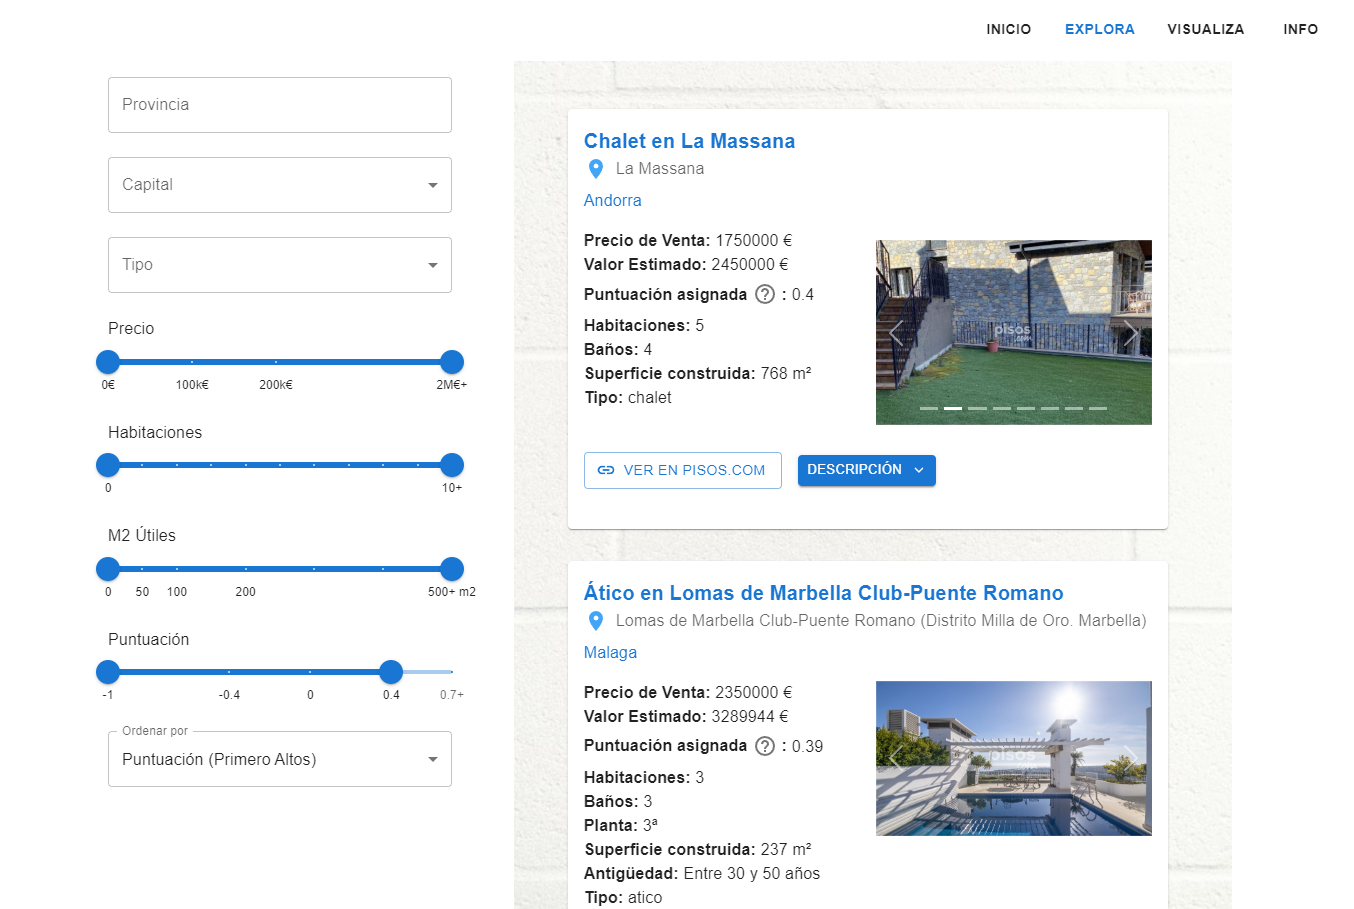
\includegraphics[width=1\textwidth]{img/explora_1.PNG}
	\caption{Vista general de página EXPLORA en \url{www.buscahogar.es}}
	\label{fig:explora_1}
\end{figure}

\clearpage
\subsection{VISUALIZA}{\label{sec:web_visualiza}}

Esta pestaña es la zona de visualización de los datos agregados en la tabla explicada en el Apéndice \ref{subsec:pisos_dw}.

Se presentan tres zonas claramente diferenciadas, una superior con filtros para las gráficas, una media con gráfica(s) de líneas y una inferior con un gráfico de barras y un mapa. En pantallas móviles o de pequeño tamaño, los filtros superiores se repliegan, para mostrarlos hay que pulsar el icono de filtro en la parte superior derecha (Ver Figura \ref{fig:filtro_moviles}).

Los filtros son los siguientes:

\begin{itemize}
    \item Comunidad Autónoma (CA): La CA de la que se quieren ver datos. Al seleccionarla, automáticamente se seleccionan todas las Provincias de dicha CA. Selección múltiple
    \item Provincia: La Provincia de la que se quieren ver inmuebles. Selección múltiple.
    \item Capital: Si se quieren ver inmuebles solo en la capital de Provincia, fuera de la capital o indiferente.
    \item Tipo: El tipo de inmueble, puede ser indiferente. Piso, casa, apartamento...
    \item Activo: Si se quieren datos de anuncios activos, retirados/vendidos o indiferente.
\end{itemize}

En la gráficas de líneas muestran datos promediados (eje $Y$), denominados como \texttt{Medidas} en la interfaz. Se observa la evolución de dichas medidas a lo largo de los meses (eje $X$). Como máximo se pueden seleccionar tres a la vez, mostrándose tres gráficas de líneas, en las que cada línea es una CA/Provincia/Media Total. Dichos datos son los siguientes actualmente:

\begin{itemize}
    \item Precio (€)
    \item Superficie útil ($m^2$)
    \item Superficie de solar ($m^2$)
    \item Número de habitaciones (ud)
    \item Número de baños (ud)
    \item Gastos de comunidad (€)
    \item Cantidad de inmuebles (anuncios) en venta / extraídos (ud)
    \item Precio por Metro Cuadrado (€)
    \item Precio por Habitación (€)
    \item Precio por Baño (€)
\end{itemize}

En la parte inferior del gráfico (parte denominada como ``categórica''), se muestran (en \%), los valores que toman las categorías seleccionadas. 


Por ejemplo, si seleccionamos categoría \texttt{Piscina Sí (\%)} se nos muestra el \% de inmuebles de cada comunidad/provincia/media total que tienen Piscina (Ver Figura \ref{fig:visualiza_1}). En el gráfico de barras se muestra una barra con el porcentaje, y en el mapa aparece un círculo localizado en dicha provincia con área proporcional al porcentaje. Si se ha seleccionado una comunidad autónoma, en el gráfico de barras aparece la media de la comunidad autónoma y en el mapa todas las provincias de dicha comunidad autónoma.


\begin{figure}[ht]
    \centering
	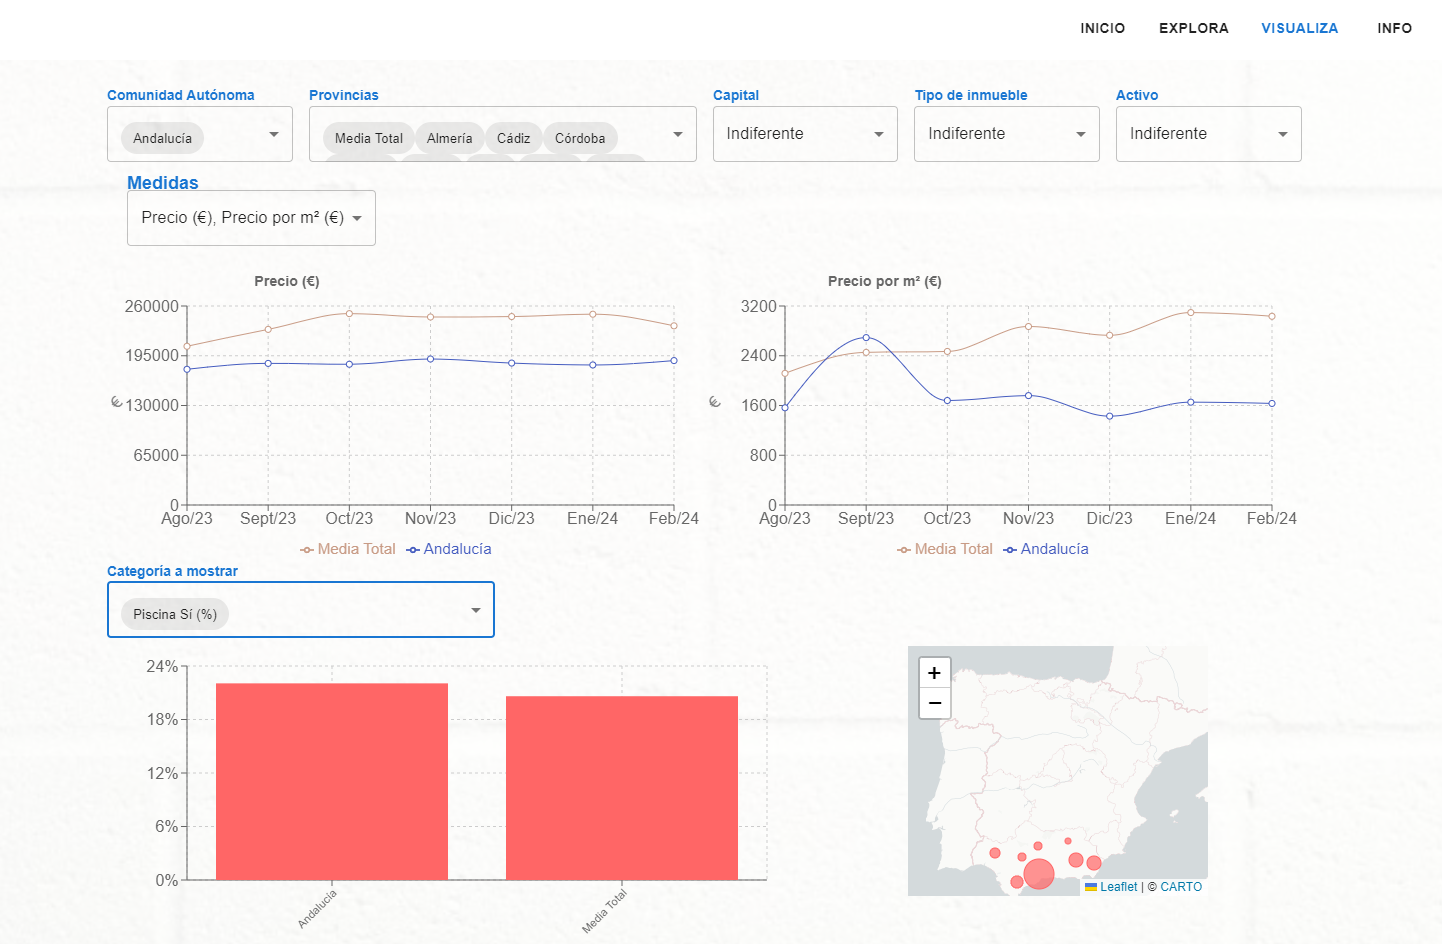
\includegraphics[width=1\textwidth]{img/visualiza_1.PNG}
	\caption[Vista general de página VISUALIZA en \url{www.buscahogar.es}]{Vista general de página VISUALIZA en \url{www.buscahogar.es}. Se ha seleccionado la comunidad autónoma Andalucía, y la categoría a mostrar \texttt{Piscina Si (\%)}}
	\label{fig:visualiza_1}
\end{figure}


\subsection{INFO}{\label{sec:web_info}}

Se trata de una sección de contacto, con el e-mail del autor principal del presente proyecto y algunas preguntas y respuestas frecuentes.

